\documentclass[aspectratio=169]{beamer}
\usetheme{Madrid}
\usecolortheme{default}

\usepackage{amsmath, amsfonts, amssymb}
\usepackage{tikz}
\usetikzlibrary{arrows.meta, calc, decorations.pathreplacing, patterns}
\usepackage{pgfplots}
\pgfplotsset{compat=1.18}

\title{Smoothing Splines}
\subtitle{Balancing Fit and Smoothness}
\author{CSE255 - Scalable Data Analysis}
\date{\today}

\begin{document}

\frame{\titlepage}

\begin{frame}{Motivation}
\begin{itemize}
    \item Given data points $(x_i, y_i)$ for $i = 1, \ldots, n$, we want to estimate a smooth function $f(x)$
    \item \textbf{Problem}: Interpolation fits exactly but may be too wiggly
    \item \textbf{Solution}: Smoothing splines balance fit quality with smoothness
    \item Trade-off: Better fit vs. smoother curve
\end{itemize}

\begin{block}{Key Idea}
Find $f$ that minimizes both the residual sum of squares and a roughness penalty
\end{block}
\end{frame}

\begin{frame}{The Smoothing Spline Problem}
Given data $(x_1, y_1), \ldots, (x_n, y_n)$ with $x_1 < x_2 < \cdots < x_n$:

\[
\min_{f} \quad \sum_{i=1}^{n} (y_i - f(x_i))^2 + \lambda \int_{x_1}^{x_n} [f''(t)]^2 \, dt
\]

\begin{itemize}
    \item \textbf{First term}: Residual sum of squares (measures fit quality)
    \item \textbf{Second term}: Roughness penalty (measures smoothness)
    \item \textbf{$\lambda$}: Smoothing parameter (controls trade-off)
    \begin{itemize}
        \item $\lambda = 0$: Interpolation (perfect fit, may be wiggly)
        \item $\lambda \to \infty$: Linear regression (smooth but may not fit well)
    \end{itemize}
\end{itemize}
\end{frame}

% --- What are cubic splines? ---
\begin{frame}{What are cubic splines?}
\begin{itemize}
    \item A \textbf{cubic spline} is a function built from \textbf{piecewise cubic polynomials}.
    \item \textbf{Knots} $x_1 < x_2 < \cdots < x_n$: the points where the pieces meet.
    \item On each interval $[x_i, x_{i+1}]$, $f(x) = a_i + b_i x + c_i x^2 + d_i x^3$ (a cubic).
    \item The pieces are \textbf{joined} so that the curve is smooth at the knots.
\end{itemize}

\begin{block}{$C_2$ continuity at knots}
At each interior knot $x_i$, we require:
\begin{itemize}
    \item $f$ is continuous (no jump)
    \item $f'$ is continuous (smooth tangent)
    \item $f''$ is continuous (smooth curvature)
\end{itemize}
So the curve has no visible ``kinks'' at the knots.
\end{block}
\end{frame}

\begin{frame}{Cubic splines: piecewise structure}
\centering
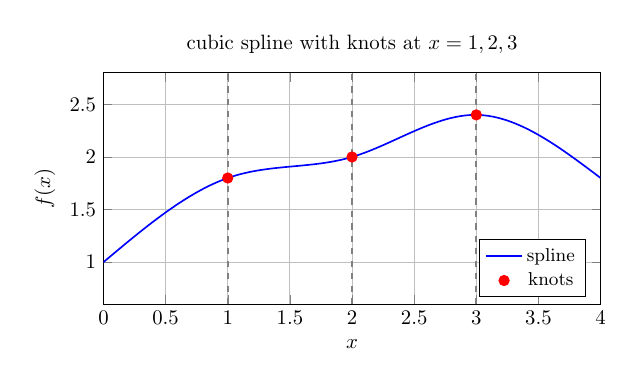
\begin{tikzpicture}[scale=0.75]
    \begin{axis}[
        width=10cm,
        height=5.5cm,
        xlabel={$x$},
        ylabel={$f(x)$},
        title={cubic spline with knots at $x = 1, 2, 3$},
        legend pos=south east,
        grid=major,
        xmin=0, xmax=4, ymin=0.6, ymax=2.8,
        legend style={font=\small}
    ]
    % Natural cubic spline: y=(1, 1.8, 2, 2.4, 1.8) at x=0,1,2,3,4. Moments M=[0, -1.157, 1.029, -1.757, 0].
    % Segment [0,1]: f(x)= 1 + 0.9928*x - 0.1928*x^3
    \addplot[domain=0:1, samples=50, thick, blue] {1 + 0.9928*x - 0.1928*x^3};
    \addlegendentry{spline}
    % [1,2]: f = M1/6*(2-x)^3 + M2/6*(x-1)^3 + (y1-M1/6)(2-x) + (y2-M2/6)(x-1)
    \addplot[domain=1:2, samples=50, thick, blue, forget plot] {-0.1928*(2-x)^3 + 0.1714*(x-1)^3 + 1.9928*(2-x) + 1.8286*(x-1)};
    % [2,3]
    \addplot[domain=2:3, samples=50, thick, blue, forget plot] {0.1714*(3-x)^3 - 0.2928*(x-2)^3 + 1.8286*(3-x) + 2.6928*(x-2)};
    % [3,4]
    \addplot[domain=3:4, samples=50, thick, blue, forget plot] {-0.2928*(4-x)^3 + 2.6928*(4-x) + 1.8*(x-3)};
    % Knots: vertical dashed lines
    \draw[dashed, gray, thick] (axis cs:1,0.6) -- (axis cs:1,2.8);
    \draw[dashed, gray, thick] (axis cs:2,0.6) -- (axis cs:2,2.8);
    \draw[dashed, gray, thick] (axis cs:3,0.6) -- (axis cs:3,2.8);
    % Knots (red points)
    \addplot[only marks, mark=*, mark size=2.5pt, red] coordinates {(1,1.8) (2,2) (3,2.4)};
    \addlegendentry{knots}
    % Knot labels
    \node[below, gray, font=\small] at (axis cs:1,0.6) {knot};
    \node[below, gray, font=\small] at (axis cs:2,0.6) {knot};
    \node[below, gray, font=\small] at (axis cs:3,0.6) {knot};
    \end{axis}
\end{tikzpicture}

\vspace{0.2cm}
\begin{itemize}
    \item \textcolor{blue}{Blue}: natural cubic spline (four cubic pieces, $C_2$ at knots). \textcolor{red}{Red}: knots.
    \item Shape goes up $\to$ dip $\to$ up $\to$ down; no kinks because $f$, $f'$, $f''$ match at each knot.
\end{itemize}
\end{frame}

\begin{frame}{Cubic splines: why cubics?}
\begin{itemize}
    \item \textbf{Linear} pieces: only $f$ continuous $\Rightarrow$ corners at knots.
    \item \textbf{Quadratic} pieces: $f$, $f'$ continuous $\Rightarrow$ smooth but curvature can jump.
    \item \textbf{Cubic} pieces: $f$, $f'$, $f''$ continuous $\Rightarrow$ smooth curve and smooth curvature (no visible break).
\end{itemize}
\end{frame}

\begin{frame}{Natural Cubic Splines}
Given data $(x_1,y_1), \ldots, (x_n,y_n)$ with $x_1 < x_2 < \cdots < x_n$.

The solution to the smoothing spline problem is a \textbf{natural cubic spline}:

\begin{block}{Definition}
A function $f$ is a natural cubic spline with knots at $x_1, \ldots, x_n$ if:
\begin{enumerate}
    \item $f$ is a cubic polynomial on each interval $[x_i, x_{i+1}]$
    \item $f$ is twice continuously differentiable at the knots
    \item $f''(x_1) = f''(x_n) = 0$ (natural boundary conditions)
\end{enumerate}
\end{block}

\begin{itemize}
    \item Natural cubic splines have $n$ degrees of freedom
    \item They provide the smoothest interpolant (minimum curvature)
    \item The solution can be computed efficiently using basis functions
\end{itemize}
\end{frame}

\begin{frame}{Basis Representation}
Any natural cubic spline can be written as:

\[
f(x) = \sum_{j=1}^{n} N_j(x) \theta_j
\]

where $N_j(x)$ are \textbf{natural cubic spline basis functions} (B-splines).

\begin{block}{Matrix Form}
\[
\mathbf{f} = \mathbf{N} \boldsymbol{\theta}
\]
where:
\begin{itemize}
    \item $\mathbf{f} = [f(x_1), \ldots, f(x_n)]^\top$
    \item $\mathbf{N}$ is the $n \times n$ basis matrix: $N_{ij} = N_j(x_i)$
    \item $\boldsymbol{\theta} = [\theta_1, \ldots, \theta_n]^\top$ are coefficients
\end{itemize}
\end{block}
\end{frame}

\begin{frame}{Natural cubic spline basis functions}
With knots $x_1 < \cdots < x_n$, the \textbf{natural cubic spline basis} $\{N_1, \ldots, N_n\}$ has one function per knot. A common choice is the \textbf{cardinal basis}: $N_j(x_i) = \delta_{ij}$ (1 at $x_j$, 0 at other knots), so $f(x_i) = \theta_i$.

\vspace{0.3cm}
\centering
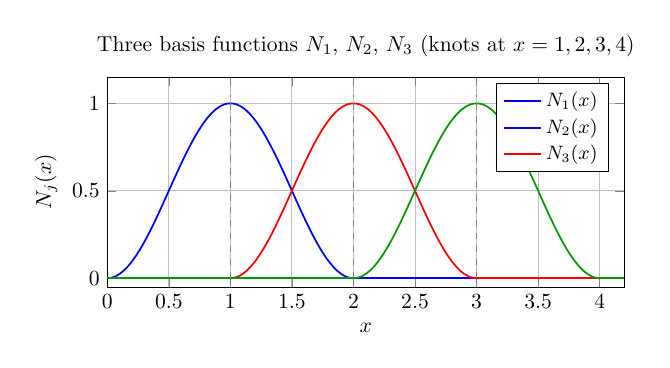
\begin{tikzpicture}[scale=0.78]
    \begin{axis}[
        width=10cm,
        height=5cm,
        xlabel={$x$},
        ylabel={$N_j(x)$},
        title={Three basis functions $N_1$, $N_2$, $N_3$ (knots at $x = 1, 2, 3, 4$)},
        legend pos=north east,
        grid=major,
        xmin=0, xmax=4.2, ymin=-0.05, ymax=1.15,
        legend style={font=\small}
    ]
    % Bump centered at 1: smooth, 0 at 0 and 2
    \addplot[domain=0:2, samples=60, thick, blue] {sin(90*x)^2};
    \addplot[domain=2:4.2, samples=40, thick, blue] {0};
    \addlegendentry{$N_1(x)$}
    % Bump centered at 2
    \addplot[domain=0:1, samples=30, thick, red, forget plot] {0};
    \addplot[domain=1:3, samples=60, thick, red] {sin(90*(x-1))^2};
    \addplot[domain=3:4.2, samples=30, thick, red, forget plot] {0};
    \addlegendentry{$N_2(x)$}
    % Bump centered at 3
    \addplot[domain=0:2, samples=30, thick, green!60!black, forget plot] {0};
    \addplot[domain=2:4, samples=60, thick, green!60!black] {sin(90*(x-2))^2};
    \addplot[domain=4:4.2, samples=10, thick, green!60!black, forget plot] {0};
    \addlegendentry{$N_3(x)$}
    \draw[dashed, gray] (axis cs:1,0) -- (axis cs:1,1.05);
    \draw[dashed, gray] (axis cs:2,0) -- (axis cs:2,1.05);
    \draw[dashed, gray] (axis cs:3,0) -- (axis cs:3,1.05);
    \end{axis}
\end{tikzpicture}

\vspace{0.2cm}
\small
Each $N_j$ is a natural cubic spline: smooth ($C_2$), nonzero mainly near $x_j$, and $N_j(x_i) = 0$ for $i \neq j$, $N_j(x_j) = 1$.
\end{frame}

\begin{frame}{Linear combination of basis functions}
Any natural cubic spline $f$ is a weighted sum: $f(x) = \sum_{j=1}^n \theta_j N_j(x)$. The coefficients $\theta_j$ are the values at the knots: $\theta_j = f(x_j)$ (for the cardinal basis).

\vspace{0.25cm}
\centering
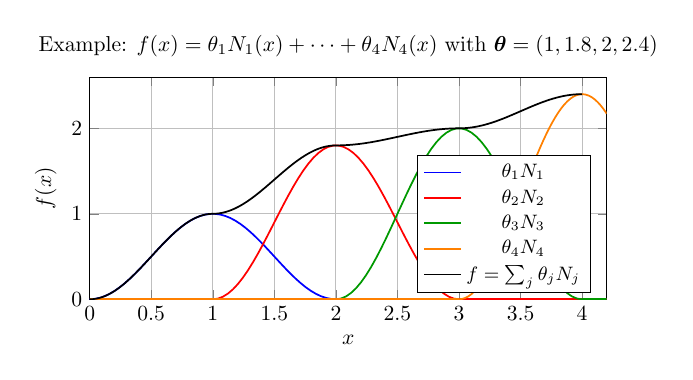
\begin{tikzpicture}[scale=0.78]
    \begin{axis}[
        width=10cm,
        height=5.2cm,
        xlabel={$x$},
        ylabel={$f(x)$},
        title={Example: $f(x) = \theta_1 N_1(x) + \cdots + \theta_4 N_4(x)$ with $\boldsymbol{\theta} = (1, 1.8, 2, 2.4)$},
        legend pos=south east,
        grid=major,
        xmin=0, xmax=4.2, ymin=0, ymax=2.6,
        legend style={font=\small}
    ]
    % Four bumps scaled by theta; knots at 1,2,3,4
    \addplot[domain=0:2, samples=50, thick, blue] {1*sin(90*x)^2};
    \addlegendentry{$\theta_1 N_1$}
    \addplot[domain=2:4.2, samples=30, thick, blue, forget plot] {0};
    \addplot[domain=0:1, samples=20, thick, blue, forget plot] {0};
    \addplot[domain=1:3, samples=50, thick, red] {1.8*sin(90*(x-1))^2};
    \addlegendentry{$\theta_2 N_2$}
    \addplot[domain=0:1, samples=20, thick, red, forget plot] {0};
    \addplot[domain=3:4.2, samples=30, thick, red, forget plot] {0};
    \addplot[domain=2:4, samples=50, thick, green!60!black] {2*sin(90*(x-2))^2};
    \addlegendentry{$\theta_3 N_3$}
    \addplot[domain=0:2, samples=30, thick, green!60!black, forget plot] {0};
    \addplot[domain=4:4.2, samples=10, thick, green!60!black, forget plot] {0};
    \addplot[domain=3:4.2, samples=50, thick, orange] {2.4*sin(90*(x-3))^2};
    \addlegendentry{$\theta_4 N_4$}
    \addplot[domain=2:3, samples=20, thick, orange, forget plot] {0};
    \addplot[domain=0:3, samples=30, thick, orange, forget plot] {0};
    % Sum: f(x) = sum of scaled basis functions
    \addplot[domain=0:1, samples=40, thick, black] {1*sin(90*x)^2};
    \addplot[domain=1:2, samples=40, thick, black, forget plot] {1*sin(90*x)^2 + 1.8*sin(90*(x-1))^2};
    \addplot[domain=2:3, samples=40, thick, black, forget plot] {1.8*sin(90*(x-1))^2 + 2*sin(90*(x-2))^2};
    \addplot[domain=3:4, samples=40, thick, black, forget plot] {2*sin(90*(x-2))^2 + 2.4*sin(90*(x-3))^2};
    \addlegendentry{$f = \sum_j \theta_j N_j$}
    \end{axis}
\end{tikzpicture}

\vspace{0.15cm}
\small
Black curve: $f(x)$ as the sum of the scaled basis functions; at each knot $x_j$, $f(x_j) = \theta_j$.
\end{frame}

\begin{frame}{Penalized least squares: objective}
Recall: $f(x) = \sum_{j=1}^n \theta_j N_j(x) = \mathbf{N}\boldsymbol{\theta}$ at the data points. The smoothing spline problem in matrix form:

\[
\min_{\boldsymbol{\theta}} \quad \underbrace{\|\mathbf{y} - \mathbf{N}\boldsymbol{\theta}\|^2}_{\text{RSS (fit)}} + \lambda \underbrace{\int_{x_1}^{x_n} [f''(t)]^2 \, dt}_{\text{roughness}}
\]

Since $f''(t) = \sum_{j=1}^n \theta_j N_j''(t)$, the roughness term becomes a quadratic form in $\boldsymbol{\theta}$:

\[
\int_{x_1}^{x_n} [f''(t)]^2 \, dt = \sum_{i,j} \theta_i \theta_j \int_{x_1}^{x_n} N_i''(t) N_j''(t) \, dt = \boldsymbol{\theta}^\top \boldsymbol{\Omega} \boldsymbol{\theta}
\]

So we minimize:
\[
\|\mathbf{y} - \mathbf{N}\boldsymbol{\theta}\|^2 + \lambda \, \boldsymbol{\theta}^\top \boldsymbol{\Omega} \boldsymbol{\theta}
\]
\end{frame}

\begin{frame}{The penalty matrix $\boldsymbol{\Omega}$}
The \textbf{penalty matrix} $\boldsymbol{\Omega}$ is the $n \times n$ matrix with entries:
\[
\Omega_{ij} = \int_{x_1}^{x_n} N_i''(t) \, N_j''(t) \, dt
\]

\begin{itemize}
    \item \textbf{Interpretation}: inner product of second derivatives of the basis functions. Large $\Omega_{ij}$ when $N_i''$ and $N_j''$ are “aligned” (same sign over much of the interval).
    \item \textbf{Symmetric}: $\Omega_{ij} = \Omega_{ji}$.
    \item \textbf{Positive semi-definite}: $\boldsymbol{\theta}^\top \boldsymbol{\Omega} \boldsymbol{\theta} \geq 0$; it measures “total curvature” of $f = \sum \theta_j N_j$.
    \item \textbf{Effect}: penalizes coefficients that produce a wiggly $f$; larger $\lambda$ pushes $\boldsymbol{\theta}$ toward vectors in the null space of $\boldsymbol{\Omega}$ (e.g.\ linear functions).
\end{itemize}
\end{frame}

\begin{frame}{Penalized least squares: solution}
Differentiating the objective in $\boldsymbol{\theta}$ gives the \textbf{normal equations}:
\[
(\mathbf{N}^\top \mathbf{N} + \lambda \boldsymbol{\Omega}) \, \boldsymbol{\theta} = \mathbf{N}^\top \mathbf{y}
\]

\begin{block}{Solution}
\[
\hat{\boldsymbol{\theta}} = (\mathbf{N}^\top \mathbf{N} + \lambda \boldsymbol{\Omega})^{-1} \mathbf{N}^\top \mathbf{y}, \qquad
\hat{\mathbf{f}} = \mathbf{N} \hat{\boldsymbol{\theta}} = \mathbf{S}_\lambda \mathbf{y}
\]
where $\mathbf{S}_\lambda = \mathbf{N}(\mathbf{N}^\top \mathbf{N} + \lambda \boldsymbol{\Omega})^{-1} \mathbf{N}^\top$ is the \textbf{smoothing matrix} (hat matrix).
\end{block}

\begin{itemize}
    \item $\mathbf{S}_\lambda$ is symmetric, positive definite (for $\lambda > 0$).
    \item Fitted values $\hat{\mathbf{f}}$ are a linear function of $\mathbf{y}$; effective degrees of freedom $\text{df}_\lambda = \text{tr}(\mathbf{S}_\lambda)$.
\end{itemize}
\end{frame}

\begin{frame}{Notation and effective degrees of freedom}
\begin{block}{Definitions}
\begin{itemize}
    \item $\mathbf{y} = (y_1, \ldots, y_n)^\top$: \textbf{observed response} at the design points $x_1, \ldots, x_n$.
    \item $\hat{\boldsymbol{\theta}} = (\mathbf{N}^\top \mathbf{N} + \lambda \boldsymbol{\Omega})^{-1} \mathbf{N}^\top \mathbf{y}$: \textbf{estimated basis coefficients}; the solution of the penalized least squares problem.
    \item $\hat{\mathbf{f}} = \mathbf{N} \hat{\boldsymbol{\theta}} = \mathbf{S}_\lambda \mathbf{y}$: \textbf{fitted values}; $\hat{f}(x_i) = \hat{f}_i$ is the spline evaluated at $x_i$.
\end{itemize}
\end{block}

The \textbf{effective degrees of freedom} is the trace of the smoothing matrix:
\[
\text{df}_\lambda = \text{tr}(\mathbf{S}_\lambda)
\]
It counts how many “parameters” the fit effectively uses (between $2$ and $n$).
\end{frame}

\begin{frame}{Effective degrees of freedom: interpretation}
\[
\text{df}_\lambda = \text{tr}(\mathbf{S}_\lambda)
\]

\begin{itemize}
    \item Measures the effective number of parameters used by the smoother
    \item $\text{df}_\lambda = n$ when $\lambda = 0$ (interpolation: fit passes through every $y_i$)
    \item $\text{df}_\lambda = 2$ when $\lambda \to \infty$ (linear fit: straight line)
    \item Often easier to specify $\text{df}_\lambda$ than $\lambda$ directly (e.g.\ “fit with 5 df”)
\end{itemize}

\begin{block}{Relationship}
\[
\text{df}_\lambda = \sum_{i=1}^{n} \frac{1}{1 + \lambda d_i}
\]
where $d_i$ are eigenvalues of $\boldsymbol{\Omega}$ relative to $\mathbf{N}^\top \mathbf{N}$
\end{block}
\end{frame}

\begin{frame}{Effect of Smoothing Parameter}
\centering
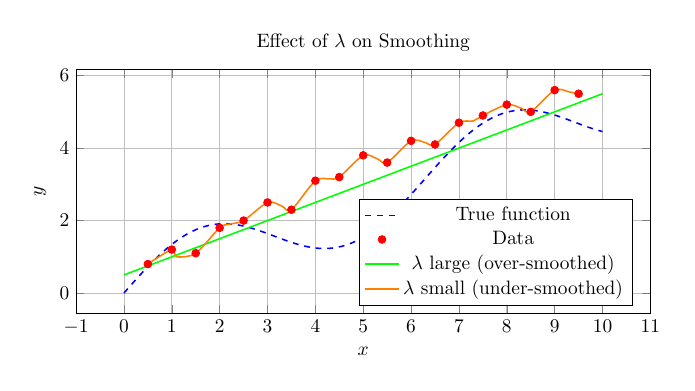
\begin{tikzpicture}[scale=0.7]
    % Generate some noisy data
    \begin{axis}[
        width=12cm,
        height=6cm,
        xlabel={$x$},
        ylabel={$y$},
        title={Effect of $\lambda$ on Smoothing},
        legend pos=south east,
        grid=major
    ]
    % True function (sine wave)
    \addplot[domain=0:10, samples=100, thick, blue, dashed] {sin(deg(x)) + 0.5*x};
    \addlegendentry{True function}
    
    % Data points
    \addplot[only marks, mark=*, mark size=2pt, red] coordinates {
        (0.5, 0.8) (1.0, 1.2) (1.5, 1.1) (2.0, 1.8) (2.5, 2.0)
        (3.0, 2.5) (3.5, 2.3) (4.0, 3.1) (4.5, 3.2) (5.0, 3.8)
        (5.5, 3.6) (6.0, 4.2) (6.5, 4.1) (7.0, 4.7) (7.5, 4.9)
        (8.0, 5.2) (8.5, 5.0) (9.0, 5.6) (9.5, 5.5)
    };
    \addlegendentry{Data}
    
    % Over-smoothed (lambda large)
    \addplot[domain=0:10, samples=100, thick, green] {0.5*x + 0.5};
    \addlegendentry{$\lambda$ large (over-smoothed)}
    
    % Under-smoothed (lambda small) - wiggly
    \addplot[domain=0:10, samples=100, thick, orange, smooth] coordinates {
        (0.5, 0.8) (1.0, 1.2) (1.1, 1.0) (1.5, 1.1) (2.0, 1.8) (2.2, 1.9)
        (2.5, 2.0) (3.0, 2.5) (3.3, 2.4) (3.5, 2.3) (4.0, 3.1) (4.3, 3.15)
        (4.5, 3.2) (5.0, 3.8) (5.3, 3.7) (5.5, 3.6) (6.0, 4.2) (6.3, 4.15)
        (6.5, 4.1) (7.0, 4.7) (7.3, 4.75) (7.5, 4.9) (8.0, 5.2) (8.3, 5.1)
        (8.5, 5.0) (9.0, 5.6) (9.3, 5.55) (9.5, 5.5)
    };
    \addlegendentry{$\lambda$ small (under-smoothed)}
    \end{axis}
\end{tikzpicture}

\begin{itemize}
    \item \textcolor{green}{Green}: Too smooth (high bias, low variance)
    \item \textcolor{orange}{Orange}: Too wiggly (low bias, high variance)
    \item \textcolor{blue}{Blue}: Optimal balance
\end{itemize}
\end{frame}

\begin{frame}{Cross-Validation for $\lambda$}
How to choose $\lambda$? Use \textbf{generalized cross-validation} (GCV):

\[
\text{GCV}(\lambda) = \frac{1}{n} \frac{\sum_{i=1}^{n} (y_i - \hat{f}_\lambda(x_i))^2}{(1 - \text{df}_\lambda/n)^2}
\]

\begin{itemize}
    \item Approximates leave-one-out cross-validation
    \item Denominator accounts for degrees of freedom
    \item Choose $\lambda$ that minimizes GCV
\end{itemize}

\begin{block}{Alternative: AIC}
\[
\text{AIC}_\lambda = n \log(\text{RSS}/n) + 2 \text{df}_\lambda
\]
\end{block}
\end{frame}

\begin{frame}{Properties of Smoothing Splines}
\begin{block}{Advantages}
\begin{itemize}
    \item \textbf{Automatic}: No need to choose knot locations
    \item \textbf{Flexible}: Can capture complex patterns
    \item \textbf{Smooth}: Continuous second derivatives
    \item \textbf{Computationally efficient}: $O(n)$ operations
    \item \textbf{Linear smoother}: $\hat{\mathbf{f}} = \mathbf{S}_\lambda \mathbf{y}$
\end{itemize}
\end{block}

\begin{block}{Limitations}
\begin{itemize}
    \item Assumes errors are independent and homoscedastic
    \item Can be sensitive to outliers
    \item May overfit with small $\lambda$ and many data points
    \item Boundary effects can occur
\end{itemize}
\end{block}
\end{frame}

\begin{frame}{Comparison with Other Methods}
\begin{columns}
\column{0.5\textwidth}
\textbf{Polynomial Regression}
\begin{itemize}
    \item Global basis
    \item Can oscillate
    \item Fixed degree
\end{itemize}

\textbf{Regression Splines}
\begin{itemize}
    \item Need to choose knots
    \item Fewer parameters
    \item Less flexible
\end{itemize}

\column{0.5\textwidth}
\textbf{Smoothing Splines}
\begin{itemize}
    \item Knots at all data points
    \item Automatic smoothing
    \item More flexible
    \item More parameters
\end{itemize}

\textbf{LOESS/LOWESS}
\begin{itemize}
    \item Local regression
    \item Window-based
    \item Good for exploration
\end{itemize}
\end{columns}
\end{frame}

\begin{frame}{Poisson GAM}
A \textbf{Generalized Additive Model} with \textbf{Poisson} response models \textbf{counts} $y_i$ (e.g.\ events in bins) with mean $\lambda_i$:

\[
\log \lambda_i = \beta_0 + f_1(x_{i1}) + f_2(x_{i2}) + \cdots
\]

\begin{itemize}
    \item \textbf{Link}: $\log$ so that $\lambda_i > 0$; each term $f_j$ is a smooth function (e.g.\ P-spline or smoothing spline).
    \item \textbf{Likelihood}: $y_i \sim \text{Poisson}(\lambda_i)$; fit by penalized maximum likelihood (smoothness penalty on the $f_j$).
    \item \textbf{Use}: event counts, rates, time-varying intensity; the smooth terms reveal how the rate depends on predictors (time of day, location, etc.).
\end{itemize}
\end{frame}

\begin{frame}{Poisson GAM for event times}
For \textbf{sequences of point events} (e.g.\ ride start times): bin time into intervals; count of events in each bin is Poisson with mean $\propto \lambda(t)$.

\begin{itemize}
    \item Model $\log \lambda(t) = \beta_0 + f(t)$ with $f(t)$ a smooth term (P-spline on hour of day). The fitted $\hat{\lambda}(t)$ is the \textbf{estimated intensity} and reveals the pattern (peaks, quiet periods).
    \item Same idea for other covariates (e.g.\ day of week, location). In pyGAM: \texttt{PoissonGAM(s(0)).fit(X, y)} with $X$ = hour (or binned time), $y$ = counts per bin.
\end{itemize}
\end{frame}

\begin{frame}{Example: Ride density throughout the day (taxi rides)}
\textbf{Data}: \textbf{timing of individual rides} at a busy station in \textbf{south Manhattan} (each ride = one event time $t$ in hours). From these event times we estimate the intensity $\lambda(t)$ so the daily \textbf{pattern} is revealed.

\vspace{0.2cm}
\small
Bins hours into intervals; count of rides in each bin is Poisson with mean $\propto \lambda(t)$. Fit a \textbf{Poisson GAM} with a P-spline on hour: $\log \lambda(t) = \beta_0 + f(t)$. The P-spline smooth reveals morning/evening rush and quiet periods.

\vspace{0.2cm}
\centering
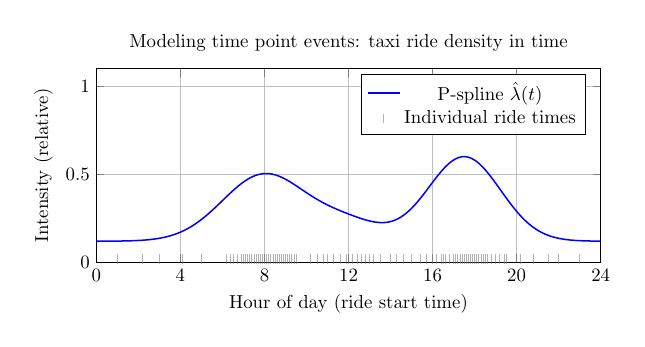
\begin{tikzpicture}[scale=0.68]
    \begin{axis}[
        width=11cm,
        height=5.2cm,
        xlabel={Hour of day (ride start time)},
        ylabel={Intensity (relative)},
        title={Modeling time point events: taxi ride density in time},
        legend pos=north east,
        grid=major,
        xmin=0, xmax=24, ymin=0, ymax=1.1,
        xtick={0,4,8,12,16,20,24}
    ]
    \addplot[domain=0:24, samples=150, thick, blue] {
        0.12 + 0.38*exp(-((x-8)^2)/8) + 0.48*exp(-((x-17.5)^2)/6) + 0.1*exp(-((x-12)^2)/5)
    };
    \addlegendentry{P-spline $\hat{\lambda}(t)$}
    \addplot[only marks, mark=|, mark size=2.5pt, mark options={thin}, gray, opacity=0.6] coordinates {
        (6.2,0.02) (6.4,0.02) (6.5,0.02) (6.7,0.02) (6.9,0.02) (7.0,0.02) (7.1,0.02) (7.2,0.02) (7.3,0.02) (7.4,0.02) (7.5,0.02) (7.6,0.02) (7.7,0.02) (7.8,0.02) (7.9,0.02) (8.0,0.02) (8.1,0.02) (8.2,0.02) (8.3,0.02) (8.4,0.02) (8.5,0.02) (8.6,0.02) (8.7,0.02) (8.8,0.02) (8.9,0.02) (9.0,0.02) (9.1,0.02) (9.2,0.02) (9.3,0.02) (9.4,0.02) (9.5,0.02)
        (10.2,0.02) (10.5,0.02) (10.8,0.02) (11.0,0.02) (11.3,0.02) (11.6,0.02) (11.9,0.02) (12.0,0.02) (12.2,0.02) (12.4,0.02) (12.6,0.02) (12.8,0.02) (13.0,0.02) (13.2,0.02) (13.5,0.02) (14.0,0.02) (14.3,0.02) (14.6,0.02) (15.0,0.02) (15.4,0.02) (15.7,0.02)
        (16.0,0.02) (16.2,0.02) (16.4,0.02) (16.5,0.02) (16.6,0.02) (16.8,0.02) (17.0,0.02) (17.1,0.02) (17.2,0.02) (17.3,0.02) (17.4,0.02) (17.5,0.02) (17.6,0.02) (17.7,0.02) (17.8,0.02) (17.9,0.02) (18.0,0.02) (18.1,0.02) (18.2,0.02) (18.3,0.02) (18.4,0.02) (18.5,0.02) (18.6,0.02) (18.8,0.02) (19.0,0.02) (19.2,0.02) (19.4,0.02) (19.5,0.02)
        (1.0,0.02) (2.2,0.02) (3.0,0.02) (4.1,0.02) (5.0,0.02) (20.2,0.02) (20.8,0.02) (21.5,0.02) (22.0,0.02) (23.0,0.02)
    };
    \addlegendentry{Individual ride times}
    \end{axis}
\end{tikzpicture}

\vspace{0.1cm}
\small
Rug: each tick = one ride start time. P-spline fit reveals intensity (morning \& evening peaks).
\end{frame}

\begin{frame}{Thin-plate splines and roughness}
\small
\textbf{Thin-plate splines}: multivariate analogue of 1D smoothing splines. Minimize $\sum_i (y_i - f(\mathbf{x}_i))^2 + \lambda J(f)$ with $\mathbf{x} \in \mathbb{R}^d$; $J(f)$ = roughness penalty in $d$ dimensions. Solution: radial basis + polynomial (``thin plate'' = bending energy of a thin sheet).

\begin{block}{Typical choices for $J(f)$}
\begin{itemize}
    \item \textbf{2D}: bending energy $\int\!\!\int \bigl( f_{xx}^2 + 2 f_{xy}^2 + f_{yy}^2 \bigr)$ (squared 2nd derivatives).
    \item \textbf{General $d$}: integral of squared mixed partials of order $m$ (e.g.\ $m{=}2$); seminorm $\|f\|^2$.
    \item \textbf{Additive}: $f = \alpha + \sum_j f_j(x_j)$ with 1D penalty per $f_j$ (avoids full thin-plate in high $d$).
\end{itemize}
\end{block}
\end{frame}

\begin{frame}{What causes the difference between the two fits?}
\small
Same data, same smoothing spline model — the \textbf{only} difference is the \textbf{smoothing parameter $\lambda$} (or equivalently effective degrees of freedom $\text{df}_\lambda$).

\begin{block}{Larger $\lambda$ (previous plot)}
Stronger penalty on roughness $\Rightarrow$ smoother fit $\Rightarrow$ only the slow annual cycle is captured (blue curve). Fewer effective degrees of freedom.
\end{block}

\begin{block}{Smaller $\lambda$ (next plot)}
Weaker penalty $\Rightarrow$ fit can follow shorter-term variation $\Rightarrow$ annual cycle plus seasonal wiggles (red curve). More effective degrees of freedom.
\end{block}

\vspace{0.2cm}
Choosing $\lambda$ (e.g.\ by GCV) trades off smoothness vs.\ fit to the data; here we show two choices to separate \textbf{trend} (blue) from \textbf{intra-seasonal variation} (red $-$ blue).
\end{frame}

\begin{frame}{Example: Weather Data Smoothing (seasonal variation)}
\small
\centering
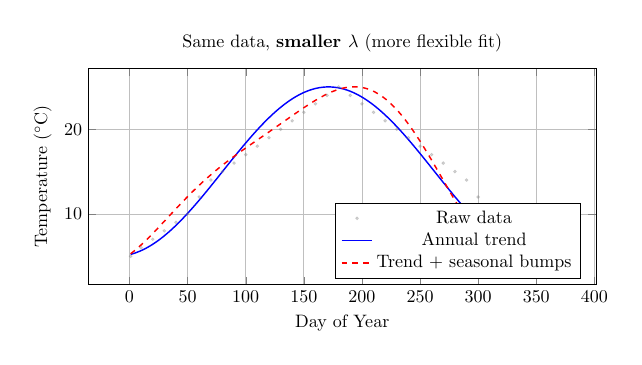
\begin{tikzpicture}[scale=0.65]
    \begin{axis}[
        width=11.5cm,
        height=5.8cm,
        xlabel={Day of Year},
        ylabel={Temperature ($^\circ$C)},
        title={Same data, \textbf{smaller $\lambda$} (more flexible fit)},
        legend pos=south east,
        grid=major
    ]
    \addplot[only marks, mark=*, mark size=0.8pt, gray, opacity=0.3] coordinates {
        (1, 5) (10, 6) (20, 7) (30, 8) (40, 9) (50, 10) (60, 12) (70, 14)
        (80, 15) (90, 16) (100, 17) (110, 18) (120, 19) (130, 20) (140, 21)
        (150, 22) (160, 23) (170, 24) (180, 25) (190, 24) (200, 23) (210, 22)
        (220, 21) (230, 20) (240, 19) (250, 18) (260, 17) (270, 16) (280, 15)
        (290, 14) (300, 12) (310, 10) (320, 9) (330, 8) (340, 7) (350, 6) (365, 5)
    };
    \addlegendentry{Raw data}
    \addplot[domain=1:365, samples=200, thick, blue] {15 + 10*sin(deg((x-80)*2*pi/365))};
    \addlegendentry{Annual trend}
    \addplot[domain=1:365, samples=200, thick, red, dashed] {15 + 10*sin(deg((x-80)*2*pi/365)) + 2*sin(deg(x*4*pi/365))};
    \addlegendentry{Trend + seasonal bumps}
    \end{axis}
\end{tikzpicture}
\vspace{-1pt}
\begin{itemize}
    \setlength{\itemsep}{2pt}
    \item \textcolor{blue}{Blue}: annual cycle. \textcolor{red}{Red}: plus \textbf{intra-seasonal} wiggles (e.g.\ warm spells, mid-season dips). Gap = variation captured by smaller $\lambda$.
\end{itemize}
\end{frame}

\begin{frame}{Applications}
\small
\setlength{\itemsep}{2pt}
\begin{columns}[T]
\column{0.33\textwidth}
\begin{block}{Time Series}
\begin{itemize}
    \item Trend extraction
    \item Seasonal decomposition
    \item Smoothing noisy data
\end{itemize}
\end{block}
\column{0.33\textwidth}
\begin{block}{Regression}
\begin{itemize}
    \item Nonparametric regression
    \item Basis for GAMs
    \item Functional data analysis
\end{itemize}
\end{block}
\column{0.33\textwidth}
\begin{block}{Visualization}
\begin{itemize}
    \item Smooth curve fitting
    \item Trend lines
    \item Exploratory analysis
\end{itemize}
\end{block}
\end{columns}
\end{frame}

\begin{frame}{Summary}
\small
\setlength{\itemsep}{3pt}
\begin{block}{Key Concepts}
\begin{itemize}
    \item Smoothing splines minimize: $\text{RSS} + \lambda \times \text{roughness}$
    \item Solution is a natural cubic spline with knots at data points
    \item $\lambda$ controls bias-variance trade-off; choose via GCV
    \item Effective degrees of freedom: $\text{df}_\lambda = \text{tr}(\mathbf{S}_\lambda)$
\end{itemize}
\end{block}
\vspace{-2pt}
\begin{block}{Takeaways}
\begin{itemize}
    \item Automatic, flexible, smooth; computationally efficient ($O(n)$)
    \item Foundation for GAMs and nonparametric regression; useful for exploration and visualization
\end{itemize}
\end{block}
\end{frame}

\begin{frame}{References and Further Reading}
\begin{itemize}
    \item Hastie, Tibshirani, Friedman. \textit{The Elements of Statistical Learning}, Chapter 5
    \item Green, Silverman. \textit{Nonparametric Regression and Generalized Linear Models}
    \item Wood, S. N. \textit{Generalized Additive Models: An Introduction with R}
    \item Reinsch, C. H. (1967). Smoothing by spline functions
\end{itemize}
\end{frame}

\end{document}

